\documentclass[paper=a4, fontsize=11pt]{scrartcl} % A4 paper and 11pt font size
\usepackage[T1]{fontenc}  % proper encoding for output file
\usepackage[utf8]{inputenc}  % except UTF-8 character in source
\usepackage[english]{babel}  % set document language
\usepackage{amsmath,amsfonts,amsthm}  % math type setting
\usepackage{mhchem}  % chemical expressions
\usepackage{graphicx}  % inclue graphics
\usepackage{url}
\usepackage{caption}
\usepackage{subcaption}
\setlength\parindent{0pt} % Removes all indentation from paragraphs

\title{Exercise 5: Jacobian and Chapman's rule}
\author{Sample Solution}
\date{\normalsize\today} 

\begin{document}

\maketitle

1. Run arts on the controlfile ``jacobian.arts''.\ \\
\ \\2. Start Matlab, run ``plot\_jacobian''. You get a figure with two sub-plots. 
One is the spectrum of nadir brightness temperature (BT) at the top of the atmosphere, the other is atmospheric zenith opacity. 
Both are for a spectral range near the 183.31 GHz water vapor line for a midlatitude-summer atmosphere.\ \\

\begin{itemize}
	\item Are there window regions?
\end{itemize}

\begin{figure}[h!]
\centering
 	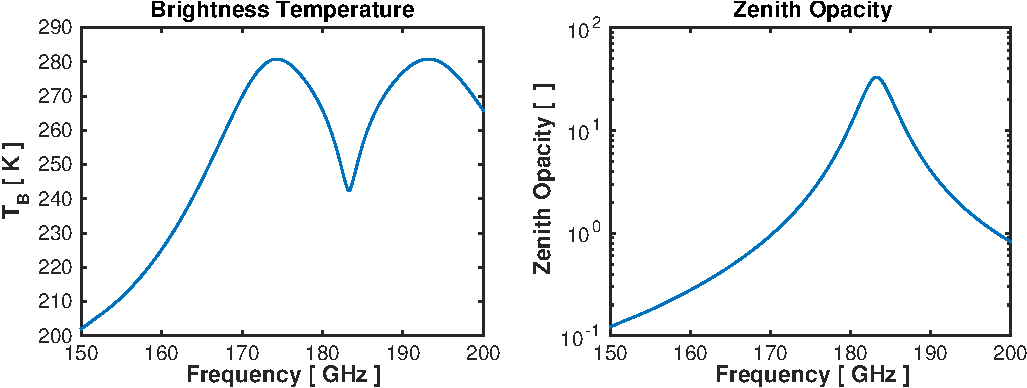
\includegraphics[width=\textwidth]{plots/bt_op_part1.pdf}
 	\caption{brightness temperature and zenith opacity}
\end{figure}

\newpage
3. The atmospheric temperature profile for the calculation was: \ \\

\begin{tabular}{rrr}
Pressure [hPa] & Temp. [K] & Altitude [km] \\
1013.000000 &	294.200000 &	0.000000 \\
902.000000 &	289.700000 &	1.000000 \\
802.000000 &	285.200000 &	2.000000 \\
710.000000 &	279.200000 &	3.000000 \\
628.000000 &	273.200000 &	4.000000 \\
554.000000 &	267.200000 &	5.000000 \\
487.000000 &	261.200000 &	6.000000 \\
426.000000 &	254.700000 &	7.000000 \\
372.000000 &	248.200000 &	8.000000 \\
324.000000 &	241.700000 &	9.000000 \\
281.000000 &	235.300000 &	10.000000 \\
243.000000 &	228.800000 &	11.000000 \\
209.000000 &	222.300000 &	12.000000 \\
179.000000 &	215.800000 &	13.000000 \\
153.000000 &	215.700000 &	14.000000 \\
130.000000 &	215.700000 &	15.000000 \\
111.000000 &	215.700000 &	16.000000 \\
95.000000 &	215.700000 &	17.000000 \\
81.200000 &	216.800000 &	18.000000 \\
69.500000 &	217.900000 &	19.000000 \\
59.500000 &	219.200000 &	20.000000 \ \\
\end{tabular}

\begin{itemize} 
	\item Where does the radiation at the peak of the line (183 GHz) originate?\ \\ -

	\item Where does the radiation at the wing (150 GHz) originate?\ \\ - 
\end{itemize}

\ \\4. Change the variable ``freq\_ind'' at the beginning of the Matlab script from -1 to a number between 1 and 110. 
This will select a frequency and mark it with a circle in the BT plot. You get two more plots, the water vapor Jacobian and the opacity between 
the top of the atmosphere and altitude z, both for the selected frequency. \ \\

\begin{itemize}
	\item Write down the altitude of the Jacobian peak and the altitude where the opacity reaches 1 for some different frequencies. \ \\ -
	
	\item Can you think of a reason why the two altitudes are not exactly the same? \ \\ -
	
	\item Explain, why the Jacobians are sometimes positive, sometimes negative. \ \\ -
\end{itemize}

\begin{figure}[h]
\centering
	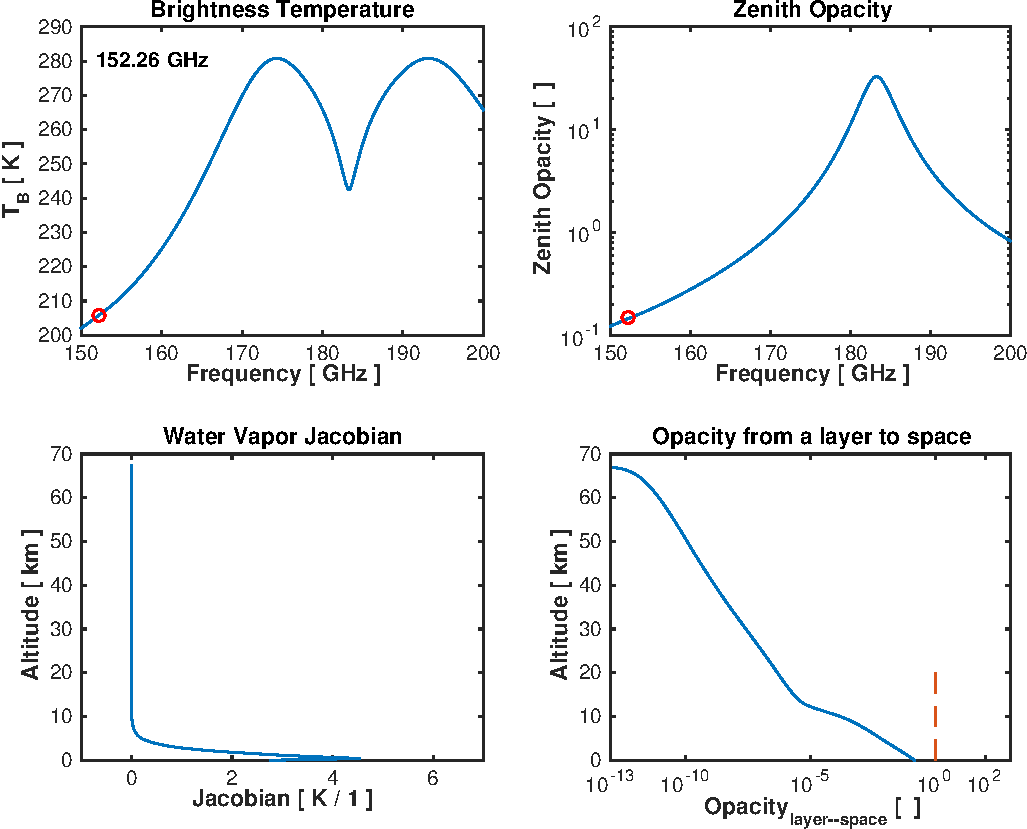
\includegraphics[width=\textwidth]{plots/jac_152GHz.pdf}
	\caption{Water vapor Jacobian and opacity between top of the atmosphere and altitude z for 152.26 GHz}
\end{figure}

\begin{figure}[h]
\centering
	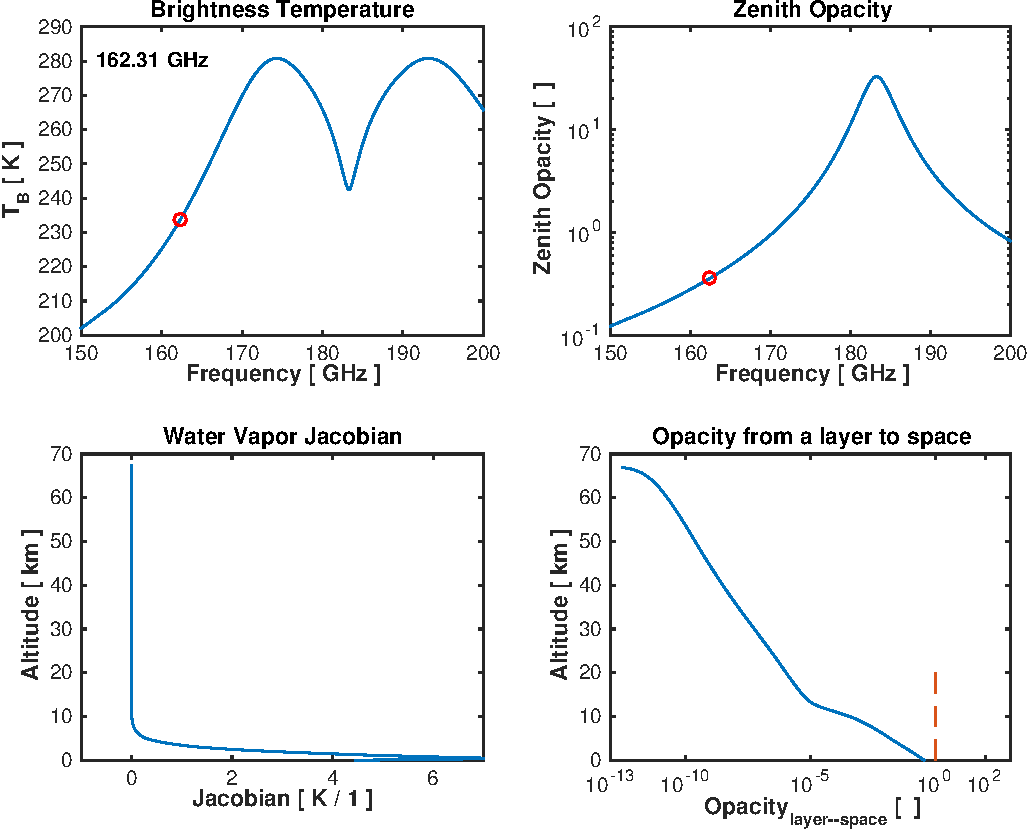
\includegraphics[width=\textwidth]{plots/jac_162GHz.pdf}
	\caption{Water vapor Jacobian and opacity between top of the atmosphere and altitude z for 167.34 GHz}
\end{figure}

\begin{figure}[h]
\centering
	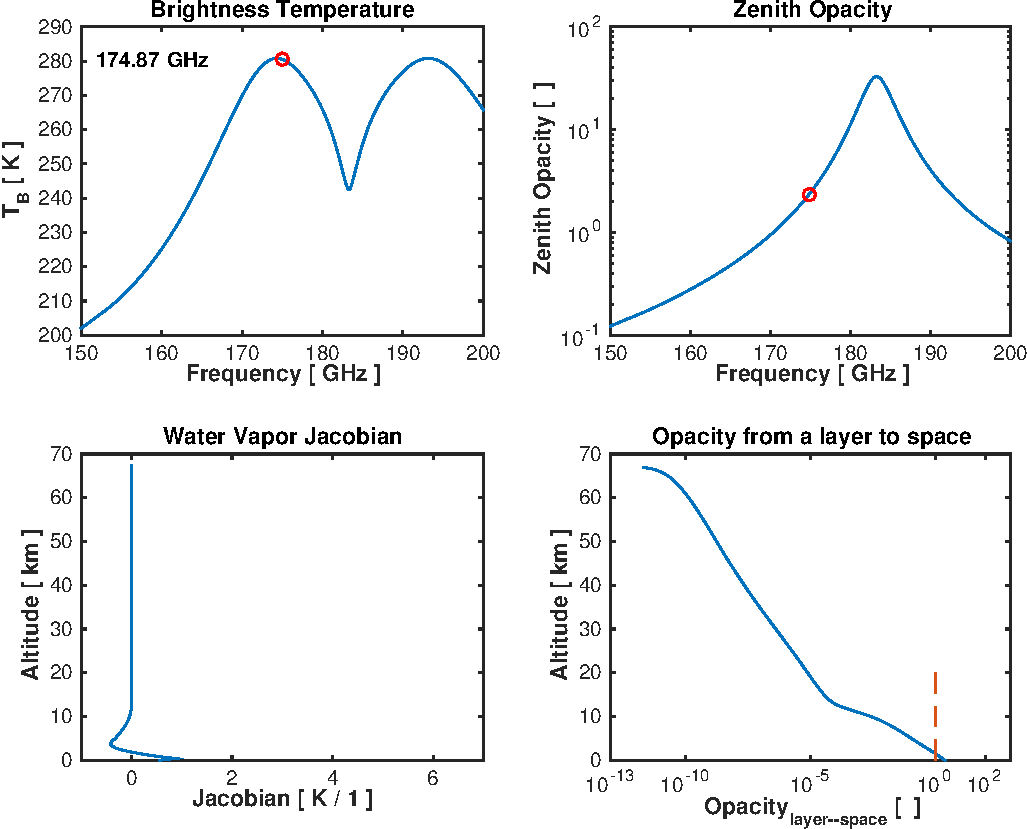
\includegraphics[width=\textwidth]{plots/jac_175GHz.pdf}
	\caption{Water vapor Jacobian and opacity between top of the atmosphere and altitude z for 179.90 GHz}
\end{figure}

\begin{figure}[h]
\centering
	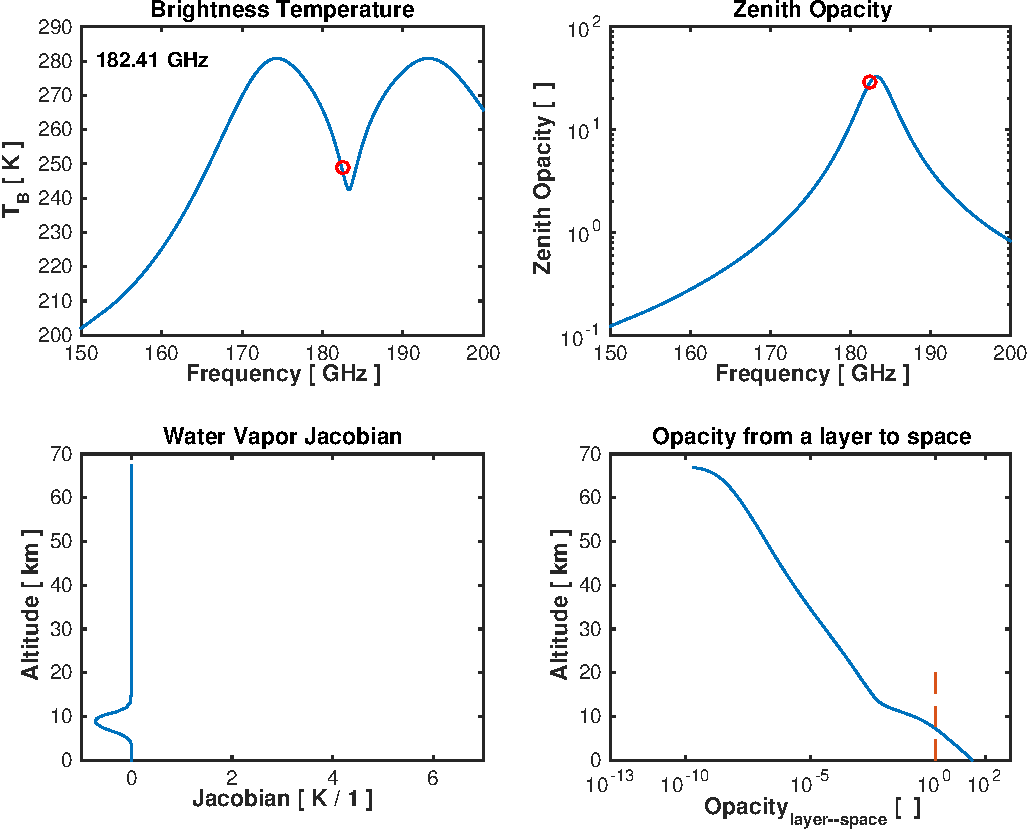
\includegraphics[width=\textwidth]{plots/jac_182GHz.pdf}
	\caption{Water vapor Jacobian and opacity between top of the atmosphere and altitude z for 182.41 GHz}
\end{figure}

\end{document}

